\documentclass[main.tex]{subfiles}
\begin{document}

\section{Sheet 11}

\subsection{Wave equation}

\subsubsection{General travelling impulse}

We want to show that any twice-differentiable function \(F(z \pm v t) = f(z, t)\) solves the wave equation: 
%
\boxalign{
\begin{align}
\qty(-\partial_{t}^2 + v^2 \partial_{z}^2) f(t, z) = 0
\,. 
\end{align}}

We denote \(\alpha (t,z) = z \pm vt\), so that \(f = F \circ \alpha \) and: 
%
\begin{subequations}
\begin{align}
\pdv[2]{f}{t} = \pdv{}{t }\qty( \dv{F}{\alpha } \pdv{\alpha }{t}) &= \dv{F}{\alpha } \pdv[2]{\alpha }{t} +  \pdv{\alpha }{t} \pdv{}{t} \qty(\dv{F}{\alpha })  \\
&= \dv{F}{\alpha } \pdv[2]{\alpha }{t}
+ \pdv{\alpha }{t}\dv{}{\alpha } \qty(\dv{F}{\alpha } \pdv[]{\alpha }{t}) \marginnote{Commuted the derivatives}\\
&= \dv{F}{\alpha } \pdv[2]{\alpha }{t}
+ \pdv{\alpha }{t} \qty( \dv[2]{F}{\alpha } \pdv[]{\alpha }{t} 
+ \dv{F}{\alpha } \cancelto{}{\pdv{}{t} \dv{\alpha }{\alpha }}) \marginnote{Derivative of a constant}  \\
&= \dv{F}{\alpha } \pdv[2]{\alpha }{t}
+ \dv[2]{F}{\alpha } \qty(\pdv[]{\alpha }{t})^2  \label{eq:faa-di-bruno}\\
&= v^2 \dv[2]{F}{\alpha }
\,,
\end{align}
\end{subequations}
%
where the expression we derived is fully general up to equation \eqref{eq:faa-di-bruno}, while the last passage comes from the fact that \(\pdv*{\alpha }{t} = \pm v\), so its square is \(v^2\) while the second derivative is zero since \(v\) is a constant. By the same reasoning, 
%
\begin{subequations}
\begin{align}
\pdv[2]{f}{z} &= \dv{F}{\alpha } \pdv[2]{\alpha }{z} 
+ \dv[2]{F}{\alpha } \qty(\pdv{\alpha }{z})^2  \\
&= \dv[2]{F}{\alpha }
\,.
\end{align}
\end{subequations}

Therefore, 
%
\begin{align}
\qty(-\partial_{t}^2 + v^2 \partial_{z}^2) f(t, z) 
= (-v^2 + v^2) \dv[2]{F}{\alpha } \equiv 0 
\,.
\end{align}

\subsubsection{Gaussian pulse}

At any fixed time \(t\), the function 
%
\begin{align}
F(\alpha ) = \exp(- \alpha^2) = \exp(- \qty(z - v t)^2)
\,
\end{align}
%
looks like a rescaled Gaussian, centered around \(z = vt\). A plot of this, with \(v = 6\) and \(t = 0, 1, 2\) is shown in figure \ref{fig:moving-gaussian-pulse}.

\begin{figure}[H]
\centering
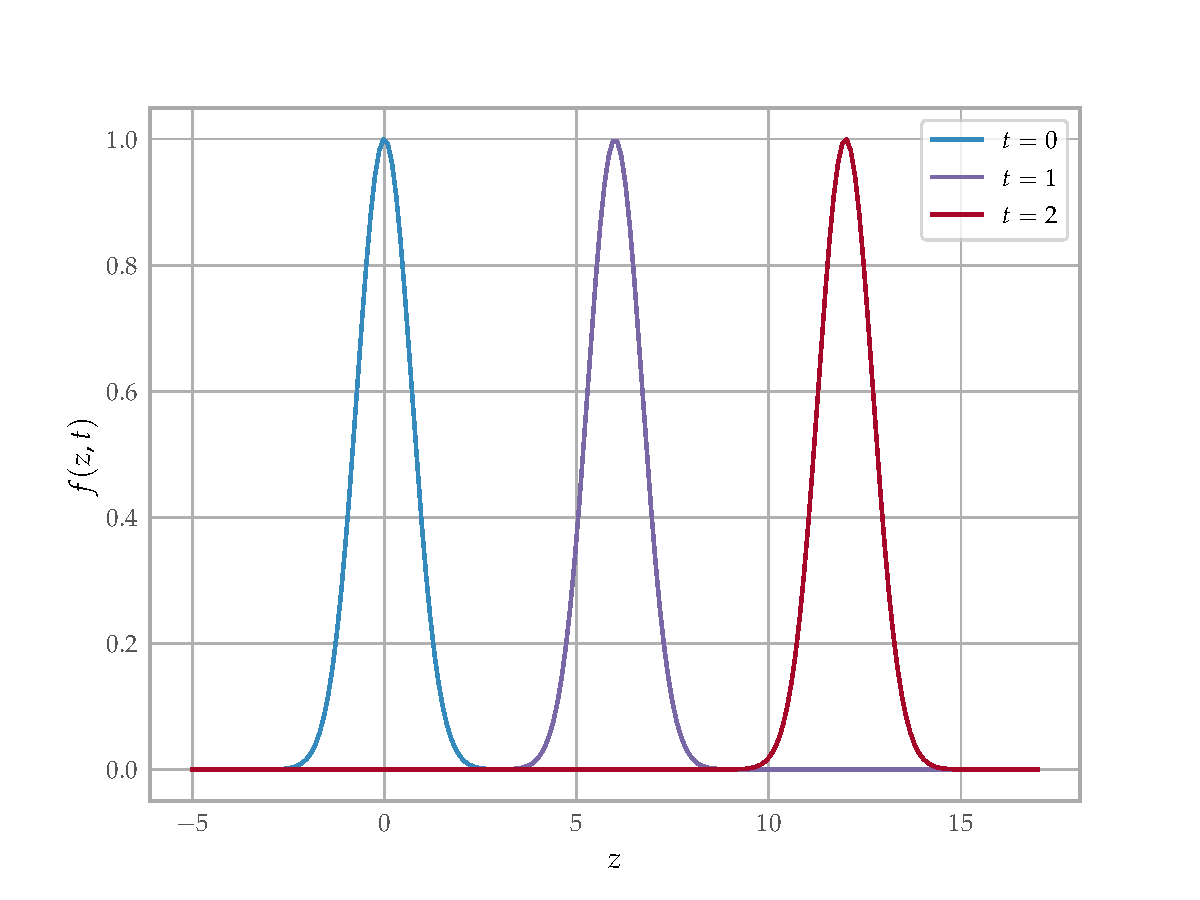
\includegraphics[width=\textwidth]{figures/gauss.pdf}
\caption{Pulse for \(t = 0, 1, 2\).}
\label{fig:moving-gaussian-pulse}
\end{figure}

\subsection{Gravitational waves}

\end{document}